%%
%%

\section*{The Windows Version of Bacula}
\label{_ChapterStart7}
\index[general]{Windows Version of Bacula }
\addcontentsline{toc}{section}{Windows Version of Bacula}

\subsection*{General}
\index[general]{General }
\addcontentsline{toc}{subsection}{General}

At the current time only the File daemon or Client program has been tested on
Windows. As a consequence, when we speak of the Windows version of Bacula
below, we are referring to the File daemon only. 

The Windows version of the Bacula File daemon has been tested on Win98, WinMe,
WinNT, and Win2000 systems. We have coded to support Win95, but no longer have
a system for testing. The Windows version of Bacula is a native Win32 port,
but there are very few source code changes, which means that the Windows
version is for the most part running code that has long proved stable on Unix
systems. When running, it is perfectly integrated with Windows and displays
its icon in the system icon tray, and provides a system tray menu to obtain
additional information on how Bacula is running (status and events dialog
boxes). If so desired, it can also be stopped by using the system tray menu,
though this should normally never be necessary. 

Once installed Bacula normally runs as a system service. This means that it is
immediately started by the operating system when the system is booted, and
runs in the background even if there is no user logged into the system. 

\subsubsection*{Win32 Installation}
\label{installation}
\index[general]{Installation }
\index[general]{Win32!Installation }
\addcontentsline{toc}{subsubsection}{Win32 Installation}

Normally, you will install the Windows version of Bacula from the binaries.
This install is standard Windows .exe that runs an install wizard using the
NSIS Free Software installer, so if you have already installed Windows
software, it should be very familiar to you. 

If you have a previous version Cygwin of Bacula (1.32 or lower) installed, you
should stop the service, uninstall it, and remove the directory possibly
saving your bacula-fd.conf file for use with the new version you will install.
The new native version of Bacula has far fewer files than the old Cygwin
version. 

Finally, proceed with the installation. 

\begin{itemize}
\item Simply double click on the {\bf winbacula-1.xx.0.exe}  NSIS install
   icon. The  actual name of the icon will vary from one release version to 
   another. 


\includegraphics{./win32-nsis.eps}  winbacula-1.xx.0.exe  
\ 
\item Once launched, the installer wizard will ask you if you want  to install
   Bacula.  

\addcontentsline{lof}{figure}{Win32 Client Setup Wizard}

\includegraphics{./win32-welcome.eps}  
\ 
\item If you proceed, you will be asked to select the components to be 
   installed. You may install the Bacula program (Bacula File Service)  and or
   the documentation. Both will be installed in sub-directories  of the install
location that you choose later. The components  dialog looks like the
following:  

\addcontentsline{lof}{figure}{Win32 Component Selection Dialog}

\includegraphics{./win32-pkg.eps}  

\item Next you will be asked to select an installation directory.  

   \addcontentsline{lof}{figure}{Win32 Directory Selection Dialog}

\includegraphics{./win32-location.eps}  

\item If you are installing for the first time, you will  be asked if you want
   to edit the bacula-fd.conf file, and  if you respond with yes, it will be
   opened in notepad.  
\ 
\item Then the installer will ask if wish to install Bacula as a  service. You
   should always choose to do so:  

\addcontentsline{lof}{figure}{Win32 Client Service Selection}

\includegraphics{./win32-service.eps}  

\ 
\item If everything goes well, you will receive the following  confirmation:  

   \addcontentsline{lof}{figure}{Win32 Client Service Confirmation}

\includegraphics{./win32-service-ok.eps}  

\ 
\item Then you will be asked if you wish to start the service.  If you respond
   with yes, any running Bacula will be shutdown  and the new one started. You
   may see a DOS box momentarily  appear on the screen as the service is started.
It should  disappear in a second or two:  

\addcontentsline{lof}{figure}{Win32 Client Start}
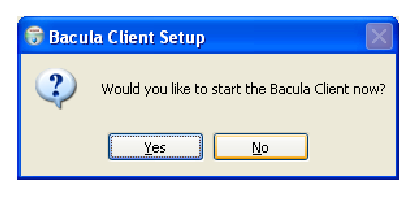
\includegraphics{./win32-start.eps}  

\ 
\item Finally, the finish dialog will appear:  

   \addcontentsline{lof}{figure}{Win32 Client Setup Completed}

\includegraphics{./win32-finish.eps}  

\ 
\end{itemize}

That should complete the installation process. When the Bacula File Server is
ready to serve files, an icon 
\includegraphics{./idle.eps} representing a
cassette (or tape) will appear in the system tray

\includegraphics{./tray-icon.eps}; right click on it and a menu will appear.
\ 
\ \ \ \ 
\includegraphics{./menu.eps}
The {\bf Events} item is currently unimplemented, by selecting the {\bf
Status} item, you can verify whether any jobs are running or not. 

When the Bacula File Server begins saving files, the color of the holes in the
cassette icon will change from white to green \includegraphics{./running.eps},
and if there is an error, the holes in the cassette icon will change to red
\includegraphics{./error.eps}. 

If you are using remote desktop connections between your windows boxes, be
warned that that tray icon does not always appear. It will always be visible
when you log into the console, but the remote desktop may not display it. 

\subsubsection*{Post Win32 Installation}
\index[general]{Post Win32 Installation }
\index[general]{Win32!Post Installation }
\addcontentsline{toc}{subsubsection}{Post Win32 Installation}

After installing Bacula and before running it, you should check the contents
of {\bf
c:\textbackslash{}bacula\textbackslash{}bin\textbackslash{}bacula-fd.conf} to
ensure that it corresponds to your configuration. 

\subsubsection*{Uninstalling Bacula on Win32}
\index[general]{Win32!Uninstalling Bacula }
\index[general]{Uninstalling Bacula on Win32 }
\addcontentsline{toc}{subsubsection}{Uninstalling Bacula on Win32}

Once Bacula has been installed, it can be uninstalled using the standard
Windows Add/Remove Programs dialog found on the Control panel. 

\subsubsection*{Dealing with Win32 Problems}
\label{problems}
\index[general]{Win32!Dealing with Problems }
\index[general]{Dealing with Win32 Problems }
\addcontentsline{toc}{subsubsection}{Dealing with Win32 Problems}

The most likely source of problems is authentication when the Director
attempts to connect to the File daemon that you installed. This can occur if
the names and the passwords defined in the File daemon's configuration file
{\bf
c:\textbackslash{}bacula\textbackslash{}bin\textbackslash{}bacula-fd.conf} on
the Windows machine do not match with the names and the passwords in the
Director's configuration file {\bf bacula-dir.conf} located on your Unix/Linux
server. 

More specifically, the password found in the {\bf Client} resource in the
Director's configuration file must be the same as the password in the {\bf
Director} resource of the File daemon's configuration file. In addition, the
name of the {\bf Director} resource in the File daemon's configuration file
must be the same as the name in the {\bf Director} resource of the Director's
configuration file. 

It is a bit hard to explain in words, but if you understand that a Director
normally has multiple Clients and a Client (or File daemon) may permit access
by multiple Directors, you can see that the names and the passwords on both
sides must match for proper authentication. 

One user had serious problems with the configuration file until he realized
that the Unix end of line conventions were used and Bacula wanted them in
Windows format. This has not been confirmed though. 

Running Unix like programs on Windows machines is a bit frustrating because
the Windows command line shell (DOS Window) is rather primitive. As a
consequence, it is not generally possible to see the debug information and
certain error messages that Bacula prints. With a bit of work, however, it is
possible. When everything else fails and you want to {\bf see} what is going
on, try the following: 

\footnotesize
\begin{verbatim}
   Start a DOS shell Window.
   cd c:\bacula\bin
   bacula-fd -t >out
   type out
\end{verbatim}
\normalsize

The {\bf -t} option will cause Bacula to read the configuration file, print
any error messages and then exit. the {\bf \gt{}} redirects the output to the
file named {\bf out}, which you can list with the {\bf type} command. 

If something is going wrong later, or you want to run {\bf Bacula} with a
debug option, you might try starting it as: 

\footnotesize
\begin{verbatim}
   bacula-fd -d 100 >out
\end{verbatim}
\normalsize

In this case, Bacula will run until you explicitly stop it, which will give
you a chance to connect to it from your Unix/Linux server. In later versions
of Bacula (1.34 on, I think), when you start the File daemon in debug mode it
can write the output to a trace file {\bf bacula.trace} in the current
directory. To enable this, before running a job, use the console, and enter: 

\footnotesize
\begin{verbatim}
   trace on
\end{verbatim}
\normalsize

then run the job, and once you have terminated the File daemon, you will find
the debug output in the {\bf bacula.trace} file. 

In addition, you should look in the System Applications log on the Control
Panel to find any Windows errors that Bacula got during the startup process. 

Finally, due to the above problems, when you turn on debugging, and specify
trace=1 on a setdebug command in the Console, Bacula will write the debug
information to the file {\bf bacula.trace} in the directory from which Bacula
is executing. 

\label{Compatibility}

\subsubsection*{Windows Compatibility Considerations}
\index[general]{Windows Compatibility Considerations }
\index[general]{Considerations!Windows Compatibility }
\addcontentsline{toc}{subsubsection}{Windows Compatibility Considerations}

If any applications are running during the backup and they have files
opened exclusively, Bacula will not be able to backup those files, so be
sure you close your applications (or tell your users to close their
applications) before the backup.  Most Microsoft applications do not open
files exclusively so that they can be backed up.  However, you will need to
experiment.  In any case, if Bacula cannot open the file, it will print an
error message, so you will always know which files were not backed up.

During backup, Bacula doesn't know about the system registry, so you will
either need to write it out to an ASCII file using {\bf regedit~~/e} or use a
program specifically designed to make a copy or backup the registry. 

In Bacula version 1.31 and later, we use Windows backup API calls by
default.  Typical of Windows, programming these special BackupRead and
BackupWrite calls is a real nightmare of complications.  The end result
gives some distinct advantages and some disadvantages.

First, the advantages are that on WinNT/2K/XP systems, the security and
ownership information is now backed up.  In addition, with the exception of
files in exclusive use by another program (a major disaster for backup
programs on Windows), Bacula can now access all system files.  This means
that when you restore files, the security and ownership information will be
restored on WinNT/2K/XP along with the data.

The disadvantage of the Windows backup API calls is that it produces
non-portable backups.  That is files and their data that are backed up on
WinNT using the native API calls (BackupRead/BackupWrite) cannot be
restored on Win95/98/Me or Unix systems.  In principle, a file backed up on
WinNT can be restored on WinXP, but this remains to be seen in practice
(not yet tested).  In addition, the stand-alone tools such as {\bf bls} and
{\bf bextract} cannot be used to retrieve the data for those files because
those tools are not available on Windows.  All restores must use the Bacula
{\bf restore} command.  This restriction is mentioned for completeness, but
in practice should not create any problems.

As a default, Bacula backs up Windows systems using the Windows API calls.
If you want to backup data on a WinNT/2K/XP system and restore it on a
Unix/Win95/98/Me system, we have provided a special {\bf portable} option
that backups the data in a portable fashion by using portable API calls.
See the \ilink{portable option}{portable} on the Include statement in a
FileSet resource in the Director's configuration chapter for the details on
setting this option.  However, using the portable option means you may have
permissions problems accessing files, and none of the security and
ownership information will be backed up or restored.  The file data can,
however, be restored on any system.

You should always be able to restore any file backed up on Unix or Win95/98/Me
to any other system. On some systems, such as WinNT/2K/XP, you may have to
reset the ownership of such restored files. Any file backed up on WinNT/2K/XP
should in principle be able to be restored to a similar system (i.e.
WinNT/2K/XP), however, I am unsure of the consequences if the owner
information and accounts are not identical on both systems. Bacula will not
let you restore files backed up on WinNT/2K/XP to any other system (i.e. Unix
Win95/98/Me) if you have used the defaults. 

Finally, if you specify the {\bf portable=yes} option on the files you back
up. Bacula will be able to restore them on any other system. However, any
WinNT/2K/XP specific security and ownership information will be lost. 

The following matrix will give you an idea of what you can expect. Thanks to
Marc Brueckner for doing the tests: 

+ 

\addcontentsline{lot}{table}{WinNT/2K/XP Restore Portability Status}
\begin{longtable}{|l|l|p{2.8in}|}
 \hline 
\multicolumn{1}{|c| }{\bf Backup OS } & \multicolumn{1}{c| }{\bf Restore OS }
& \multicolumn{1}{c| }{\bf Results  } \\
 \hline {WinMe } & {WinMe } & {Works  } \\
 \hline {WinMe } & {WinNT } & {Works (SYSTEM permissions)  } \\
 \hline {WinMe } & {WinXP } & {Works (SYSTEM permissions)  } \\
 \hline {WinMe } & {Linux } & {Works (SYSTEM permissions)  } \\
 \hline {\ } & {\ } & {\  } \\
 \hline {WinXP } & {WinXP } & {Works  } \\
 \hline {WinXP } & {WinNT } & {Works (all files OK, but got ``The data is invalid''
message)  } \\
 \hline {WinXP } & {WinMe } & {Error: Win32 data stream not supported.  } \\
 \hline {WinXP } & {WinMe } & {Works if {\bf Portable=yes} specified during backup.} \\
 \hline {WinXP } & {Linux } & {Error: Win32 data stream not supported.  } \\
 \hline {WinXP } & {Linux } & {Works if {\bf Portable=yes} specified during backup.}\\
 \hline {\ } & {\ } & {\  } \\
 \hline {WinNT } & {WinNT } & {Works  } \\
 \hline {WinNT } & {WinXP } & {Works  } \\
 \hline {WinNT } & {WinMe } & {Error: Win32 data stream not supported.  } \\
 \hline {WinNT } & {WinMe } & {Works if {\bf Portable=yes} specified during backup.}\\
 \hline {WinNT } & {Linux } & {Error: Win32 data stream not supported.  } \\
 \hline {WinNT } & {Linux } & {Works if {\bf Portable=yes} specified during backup.  }\\
 \hline {\ } & {\ } & {\  } \\
 \hline {Linux } & {Linux } & {Works  } \\
 \hline {Linux } & {WinNT } & {Works (SYSTEM permissions)  } \\
 \hline {Linux } & {WinMe } & {Works  } \\
 \hline {Linux } & {WinXP } & {Works (SYSTEM permissions) }
\\ \hline 

\end{longtable}

\subsubsection*{Windows Firewalls}
\index[general]{Firewalls!Windows }
\index[general]{Windows Firewalls }
\addcontentsline{toc}{subsubsection}{Windows Firewalls}

If you turn on the firewalling feature on Windows (default in WinXP SR2), you
are likely to find that the Bacula ports are blocked and you cannot
communicated to the other daemons. This can be deactivated through the {\bf
Security Notification} dialog, which is apparently somewhere in the {\bf
Security Center}. I don't have this on my computer, so I cannot give the exact
details. 

The command: 

\footnotesize
\begin{verbatim}
netsh firewall set opmode disable
\end{verbatim}
\normalsize

is purported to disable the firewall, but this command is not accepted on my
WinXP Home machine. 

\subsubsection*{Windows Port Usage}
\index[general]{Windows Port Usage }
\index[general]{Usage!Windows Port }
\addcontentsline{toc}{subsubsection}{Windows Port Usage}

If you want to see if the File daemon has properly opened the port and is
listening, you can enter the following command in a shell window: 

\footnotesize
\begin{verbatim}
   netstat -an | findstr 910[123]
\end{verbatim}
\normalsize

\subsubsection*{Windows Disaster Recovery}
\index[general]{Recovery!Windows Disaster }
\index[general]{Windows Disaster Recovery }
\addcontentsline{toc}{subsubsection}{Windows Disaster Recovery}

We don't currently have a good solution for disaster recovery on Windows as we
do on Linux. The main piece lacking is a Windows boot floppy or a Windows boot
CD. Microsoft releases a Windows Pre-installation Environment ({\bf WinPE})
that could possibly work, but we have not investigated it. This means that
until someone figures out the correct procedure, you must restore the OS from
the installation disks, then you can load a Bacula client and restore files.
Please don't count on using {\bf bextract} to extract files from your backup
tapes during a disaster recovery unless you have backed up those files using
the {\bf portable} option. {\bf bextract} does not run on Windows, and the
normal way Bacula saves files using the Windows API prevents the files from
being restored on a Unix machine. Once you have an operational Windows OS
loaded, you can run the File daemon and restore your user files. 

Please see 
\ilink{ Disaster Recovery of Win32 Systems}{Win3233} for the latest
suggestion, which looks very promising. 

It looks like Bart PE Builder, which creates a Windows PE (Pre-installation
Environment) Boot-CD, may be just what is needed to build a complete disaster
recovery system for Win32. This distribution can be found at 
\elink{http://www.nu2.nu/pebuilder/ }{http://www.nu2.nu/pebuilder/}. 

\subsubsection*{Windows Ownership and Permissions Problems}
\index[general]{Problems!Windows Ownership and Permissions }
\index[general]{Windows Ownership and Permissions Problems }
\addcontentsline{toc}{subsubsection}{Windows Ownership and Permissions
Problems}

If you restore files backed up from WinNT/XP/2K to an alternate directory,
Bacula may need to create some higher level directories that were not saved
(or restored). In this case, the File daemon will create them under the SYSTEM
account because that is the account that Bacula runs under as a service. As of
version 1.32f-3, Bacula creates these files with full access permission.
However, there may be cases where you have problems accessing those files even
if you run as administrator. In principle, Microsoft supplies you with the way
to cease the ownership of those files and thus change the permissions.
However, a much better solution to working with and changing Win32 permissions
is the program {\bf SetACL}, which can be found at 
\elink{http://setacl.sourceforge.net/ }{http://setacl.sourceforge.net/}. 

\subsubsection*{Manually resetting the Permissions}
\index[general]{Manually resetting the Permissions }
\index[general]{Permissions!Manually resetting the }
\addcontentsline{toc}{subsubsection}{Manually resetting the Permissions}

The following solution was provided by Dan Langille \lt{}dan at langille in
the dot org domain\gt{}. The steps are performed using Windows 2000 Server but
they should apply to most Win32 platforms. The procedure outlines how to deal
with a problem which arises when a restore creates a top-level new directory.
In this example, ``top-level'' means something like {\bf
c:\textbackslash{}src}, not {\bf c:\textbackslash{}tmp\textbackslash{}src}
where {\bf c:\textbackslash{}tmp} already exists. If a restore job specifies /
as the {\bf Where:} value, this problem will arise. 

The problem appears as a directory which cannot be browsed with Windows
Explorer. The symptoms include the following message when you try to click on
that directory: 


\includegraphics{./access-is-denied.eps} 

If you encounter this message, the following steps will change the permissions
to allow full access. 

\begin{enumerate}
\item right click on the top level directory (in this example, {\bf c:/src})
   and  select {\bf Properties}. 
\item click on the Security tab. 
\item If the following message appears, you can ignore it, and click on {\bf
   OK}. 


\includegraphics{./view-only.eps} 

You should see something like this: 

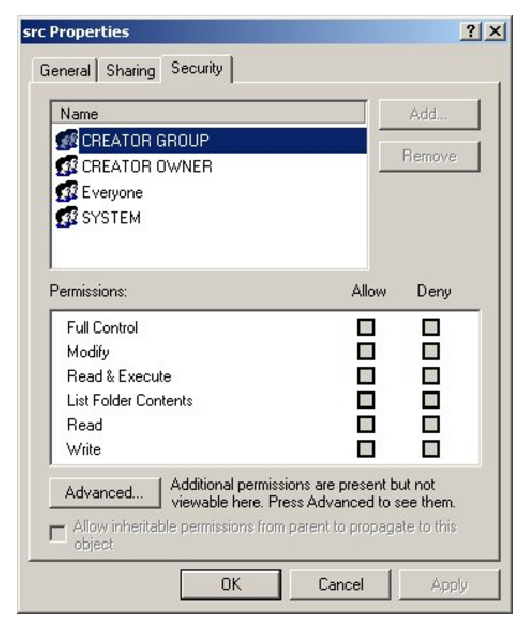
\includegraphics{./properties-security.eps} 
\item click on Advanced 
\item click on the Owner tab 
\item Change the owner to something other than the current owner (which is
   {\bf SYSTEM} in this example as shown below). 

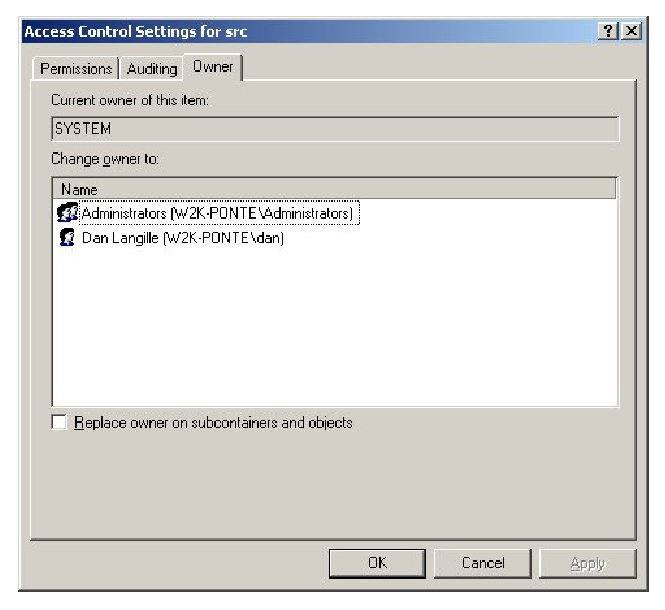
\includegraphics{./properties-security-advanced-owner.eps} 
\item ensure the ``Replace owner on subcontainers and objects'' box is 
   checked 
\item click on OK 
\item When the message ``You do not have permission to read the contents of
   directory ''c:\textbackslash{}src\textbackslash{}basis. Do you wish to replace
   the directory permissions with permissions granting you Full Control?``, click
on Yes. 


\includegraphics{./confirm.eps} 
\item Click on OK to close the Properties tab 
   \end{enumerate}

With the above procedure, you should now have full control over your restored
directory. 

\subsubsection*{Backing Up the WinNT/XP/2K System State}
\index[general]{State!Backing Up the WinNT/XP/2K System }
\index[general]{Backing Up the WinNT/XP/2K System State }
\addcontentsline{toc}{subsubsection}{Backing Up the WinNT/XP/2K System State}

A suggestion by Damian Coutts using Microsoft's NTBackup utility in
conjunction with Bacula should permit a full restore of any damaged system
files on Win2K/XP. His suggestion is to do an NTBackup of the critical system
state prior to running a Bacula backup with the following command: 

\footnotesize
\begin{verbatim}
ntbackup backup systemstate /F c:\systemstate.bkf
\end{verbatim}
\normalsize

The {\bf backup} is the command, the {\bf systemstate} says to backup only the
system state and not all the user files, and the {\bf /F
c:\textbackslash{}systemstate.bkf} specifies where to write the state file.
this file must then be saved and restored by Bacula. 

To restore the system state, you first reload a base operating system if the
OS is damaged, otherwise, this is not necessary, then you would use Bacula to
restore all the damaged or lost user's files and to recover the {\bf
c:\textbackslash{}systemstate.bkf} file. Finally if there are any damaged or
missing system files or registry problems, you run {\bf NTBackup} and {\bf
catalogue} the system statefile, and then select it for restore. The
documentation says you can't run a command line restore of the systemstate. 

To the best of my knowledge, this has not yet been tested. If you test it,
please report your results to the Bacula email list. 

\subsubsection*{Windows Considerations for Filename Specifications}
\index[general]{Specifications!Windows Considerations for Filename }
\index[general]{Windows Considerations for Filename Specifications }
\addcontentsline{toc}{subsubsection}{Windows Considerations for Filename
Specifications}

Please see the 
\ilink{Director's Configuration chapter}{win32} of this manual
for important considerations on how to specify Windows paths in Bacula FileSet
Include and Exclude directives. 

\subsubsection*{Command Line Options Specific to the Bacula Windows File
Daemon (Client)}
\index[general]{Client!Command Line Options Specific to the Bacula Windows
File Daemon }
\index[general]{Command Line Options Specific to the Bacula Windows File
Daemon (Client) }
\addcontentsline{toc}{subsubsection}{Command Line Options Specific to the
Bacula Windows File Daemon (Client)}

These options are not normally seen or used by the user, and are documented
here only for information purposes. At the current time, to change the default
options, you must either manually run {\bf Bacula} or you must manually edit
the system registry and modify the appropriate entries. 

In order to avoid option clashes between the options necessary for {\bf
Bacula} to run on Windows and the standard Bacula options, all Windows
specific options are signaled with a forward slash character (/), while as
usual, the standard Bacula options are signaled with a minus (-), or a minus
minus (\verb{--{). All the standard Bacula options can be used on the Windows
version. In addition, the following Windows only options are implemented: 

\begin{description}

\item [/servicehelper ]
   \index[fd]{/servicehelper }
   Run the service helper application  (don't use this it is deprecated.).  

\item [/service ]
   \index[fd]{/service }
   Start Bacula as a service 

\item [/run ]
   \index[fd]{/run }
   Run the Bacula application  

\item [/install ]
   \index[fd]{/install }
   Install Bacula as a service in the system registry  

\item [/remove ]
   \index[fd]{/remove }
   Uninstall Bacula from the system registry  

\item [/about ]
   \index[fd]{/about }
   Show the Bacula about dialogue box  

\item [/status ]
   \index[fd]{/status }
   Show the Bacula status dialogue box  

\item [/events ]
   \index[fd]{/events }
   Show the Bacula events dialogue box (not  yet implemented)  

\item [/kill ]
   \index[fd]{/kill }
   Stop any running {\bf Bacula}  

\item [/help ]
   \index[fd]{/help }
   Show the Bacula help dialogue box 
\end{description}

It is important to note that under normal circumstances the user should never
need to use these options as they are normally handled by the system
automatically once Bacula is installed. However, you may note these options in
some of the .bat files that have been created for your use. 

\subsubsection*{Shutting down Windows Systems}
\index[general]{Shutting down Windows Systems }
\index[general]{Systems!Shutting down Windows }
\addcontentsline{toc}{subsubsection}{Shutting down Windows Systems}

Some users like to shutdown their windows machines after a backup using a
Client Run After Job directive. If you want to do something similar, you might
take the shutdown program from the 
\elink{apcupsd project}{http://www.apcupsd.com} or one from the 
\elink{ Sysinternals
project}{http://www.sysinternals.com/ntw2k/freeware/psshutdown.shtml}. 
